\hypertarget{Beginners-Guide}{%
\chapter{Beginner's Guide}\label{Beginners-Guide}}

\hypertarget{introduction}{%
\section{Introduction}\label{introduction}}

\begin{quote}
Rigs of Rods (RoR) is a free/libre soft-body physics simulator mainly
targeted at simulating vehicle physics. The soft-body physics system is
based on mass-spring-damper theory.
\end{quote}

This page will help you learn the basics of Rigs of Rods, from
installing to playing multiplayer.

\hypertarget{first-run}{%
\section{First Run}\label{first-run}}

When launching RoR for the first time, the user directory will be
created. On Windows this is located at
\texttt{Documents\textbackslash{}Rigs\ of\ Rods\ 0.4} or at
\texttt{\textasciitilde{}/.rigsofrods} on Linux. This is where
configuration files, logs, and mods are stored.

The game should open in a small window:  

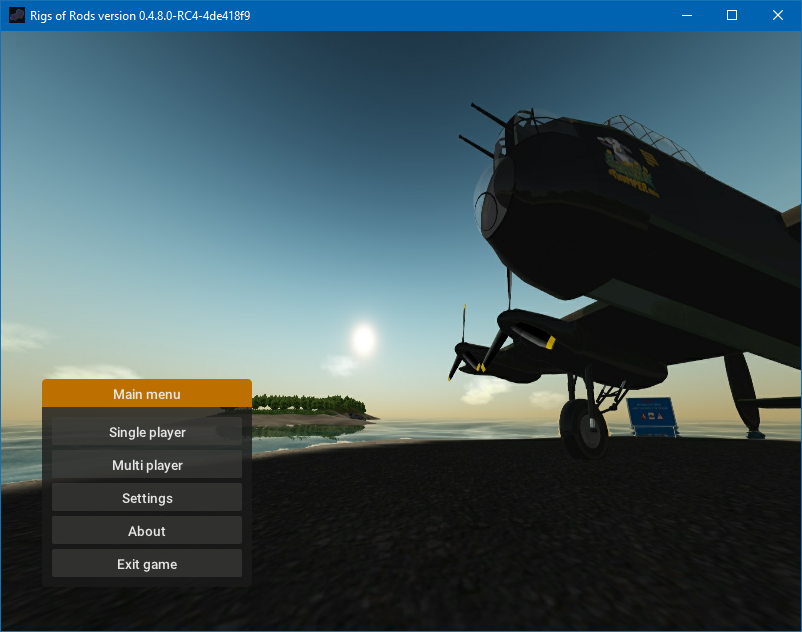
\includegraphics{images/bg-firstrun1.png}

Before playing, you should first change your settings. Begin by clicking
\texttt{Settings}.

First, make sure the rendering system is set to
\texttt{Direct3D9\ Rendering\ Subsystem}. If it's set to
\texttt{OpenGL\ Rendering\ Subsystem}, change it.

If you're running Linux, ignore this as DirectX is not available.

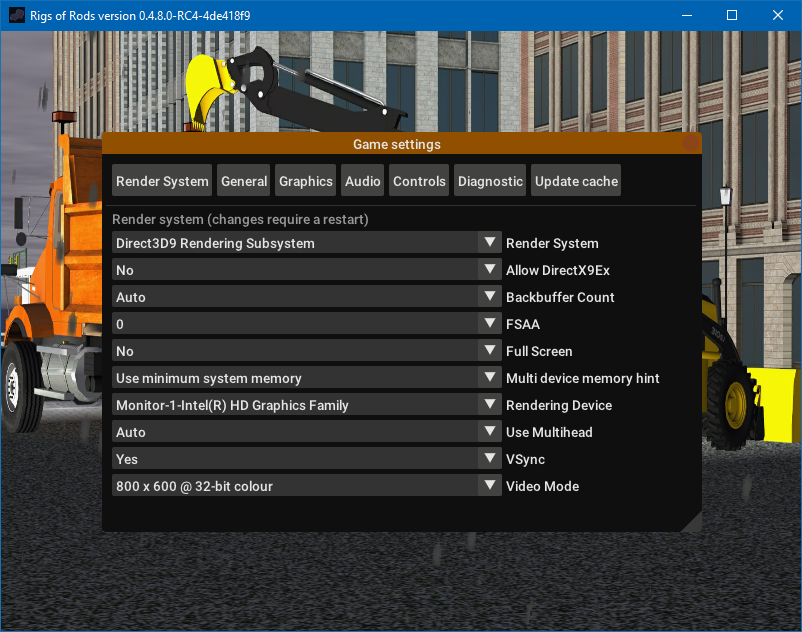
\includegraphics{images/bg-firstrun2.png}

Now select \texttt{Video\ Mode} and change it to your monitor's native
resolution then restart the game to apply your changes.


\includegraphics{images/bg-firstrun3.png}

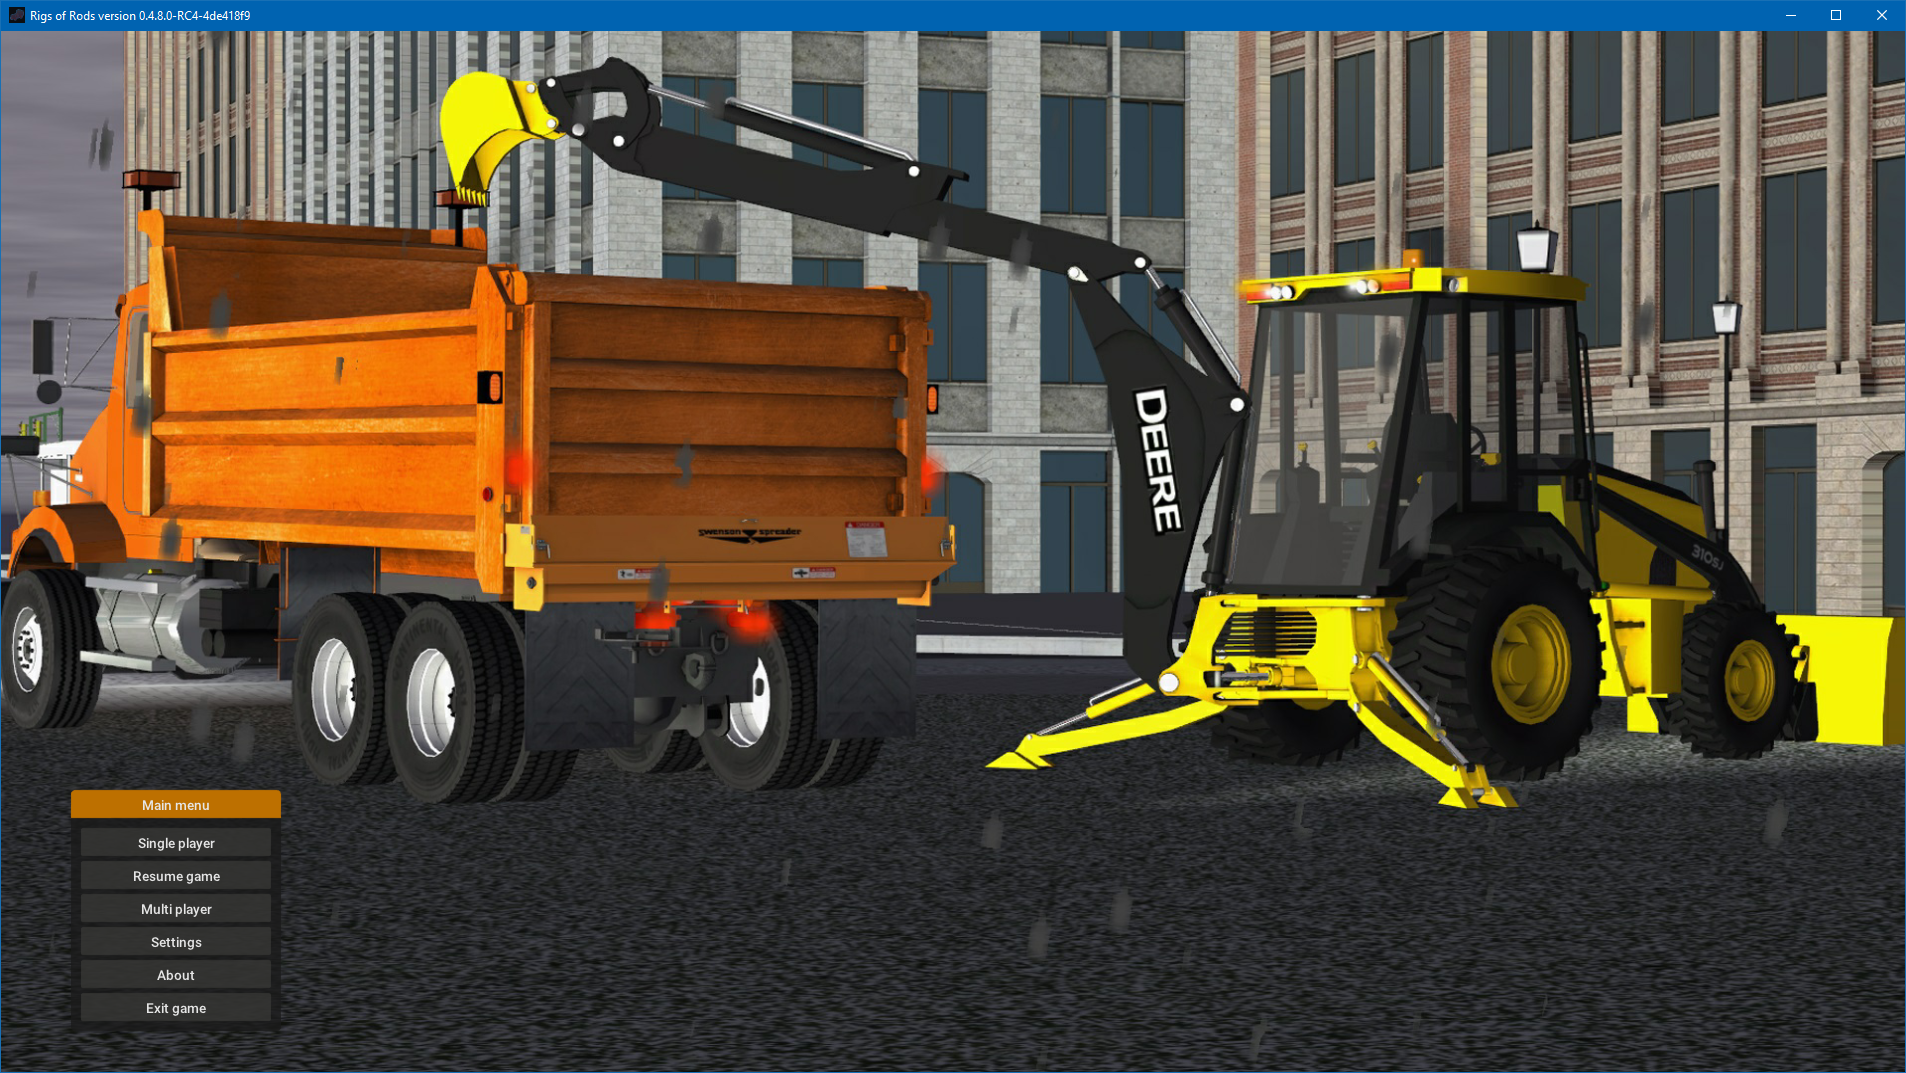
\includegraphics{images/bg-firstrun4.png}

Click \texttt{Settings} again, then click the \texttt{Graphics} tab.

The following settings should be fine for most people, but feel free to
adjust them to fit your liking.

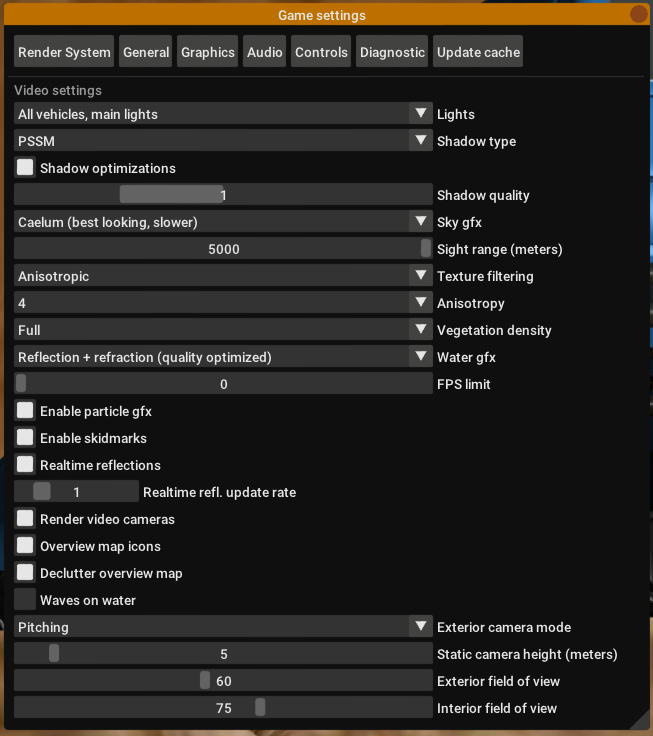
\includegraphics{images/bg-firstrun5.png}

Then click the \texttt{Audio} tab and set the volume. Due to a bug in
RC4, it is muted by default.

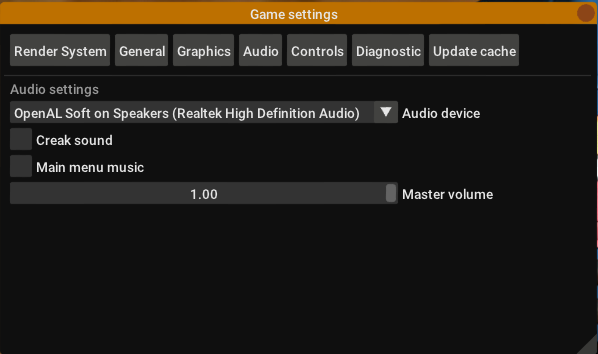
\includegraphics{images/bg-firstrun6.png}

Once you're finished, restart the game again.

Now you're ready to begin playing. Start by clicking
\texttt{Single\ player} to open the terrain selector.

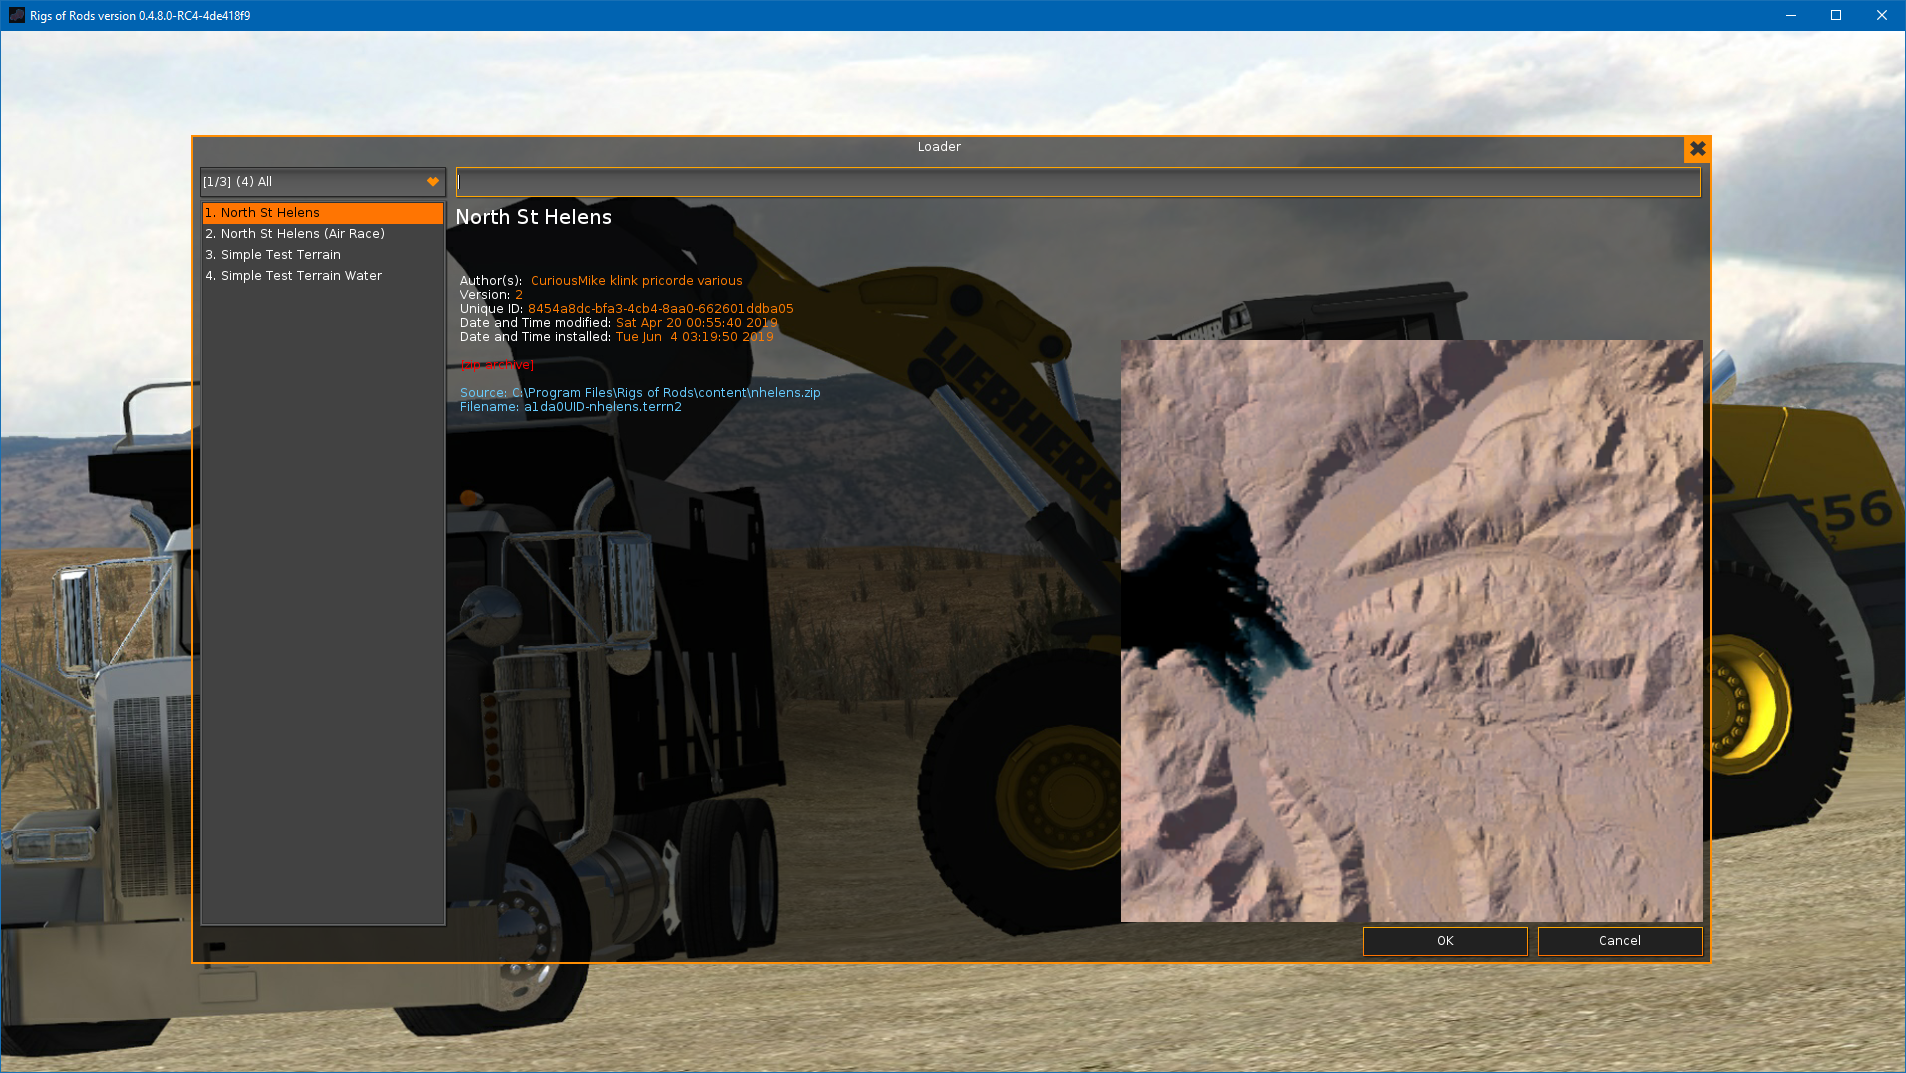
\includegraphics{images/bg-terrnselect.png}

For the sake of this tutorial, select \emph{North St Helens}.

Once the terrain loads, you will spawn as a country person known
lovingly as RoRBot. You control him with the arrow keys while using
\texttt{SHIFT} to run and \texttt{SPACE} to jump (good for getting over
bumps, or if you get stuck).

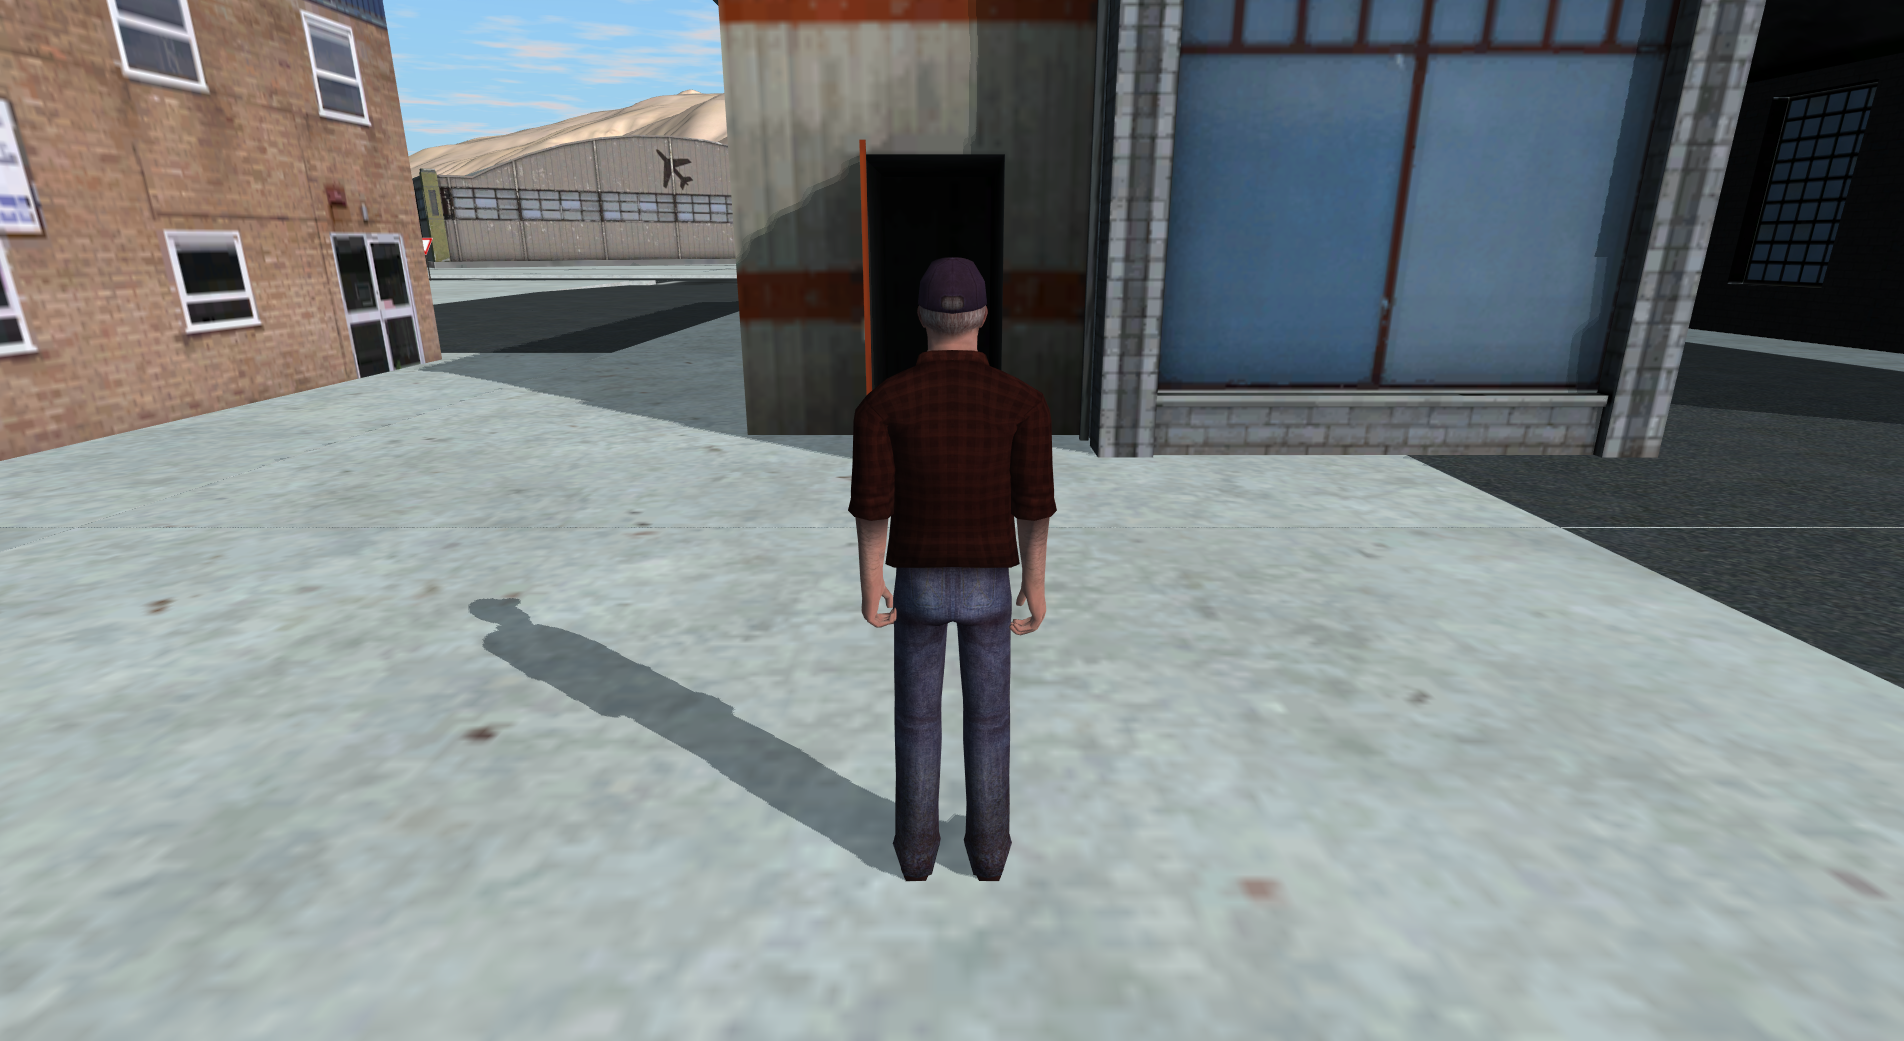
\includegraphics{images/bg-rorbot.png}

You spawn in front of a building known as the \emph{Rig-a-Deal}. This is
where you will spawn new trucks. Walk into the ``Office'' to bring up
the selection menu. You can also spawn a vehicle anywhere at any time by
pressing \texttt{CTRL+G}.

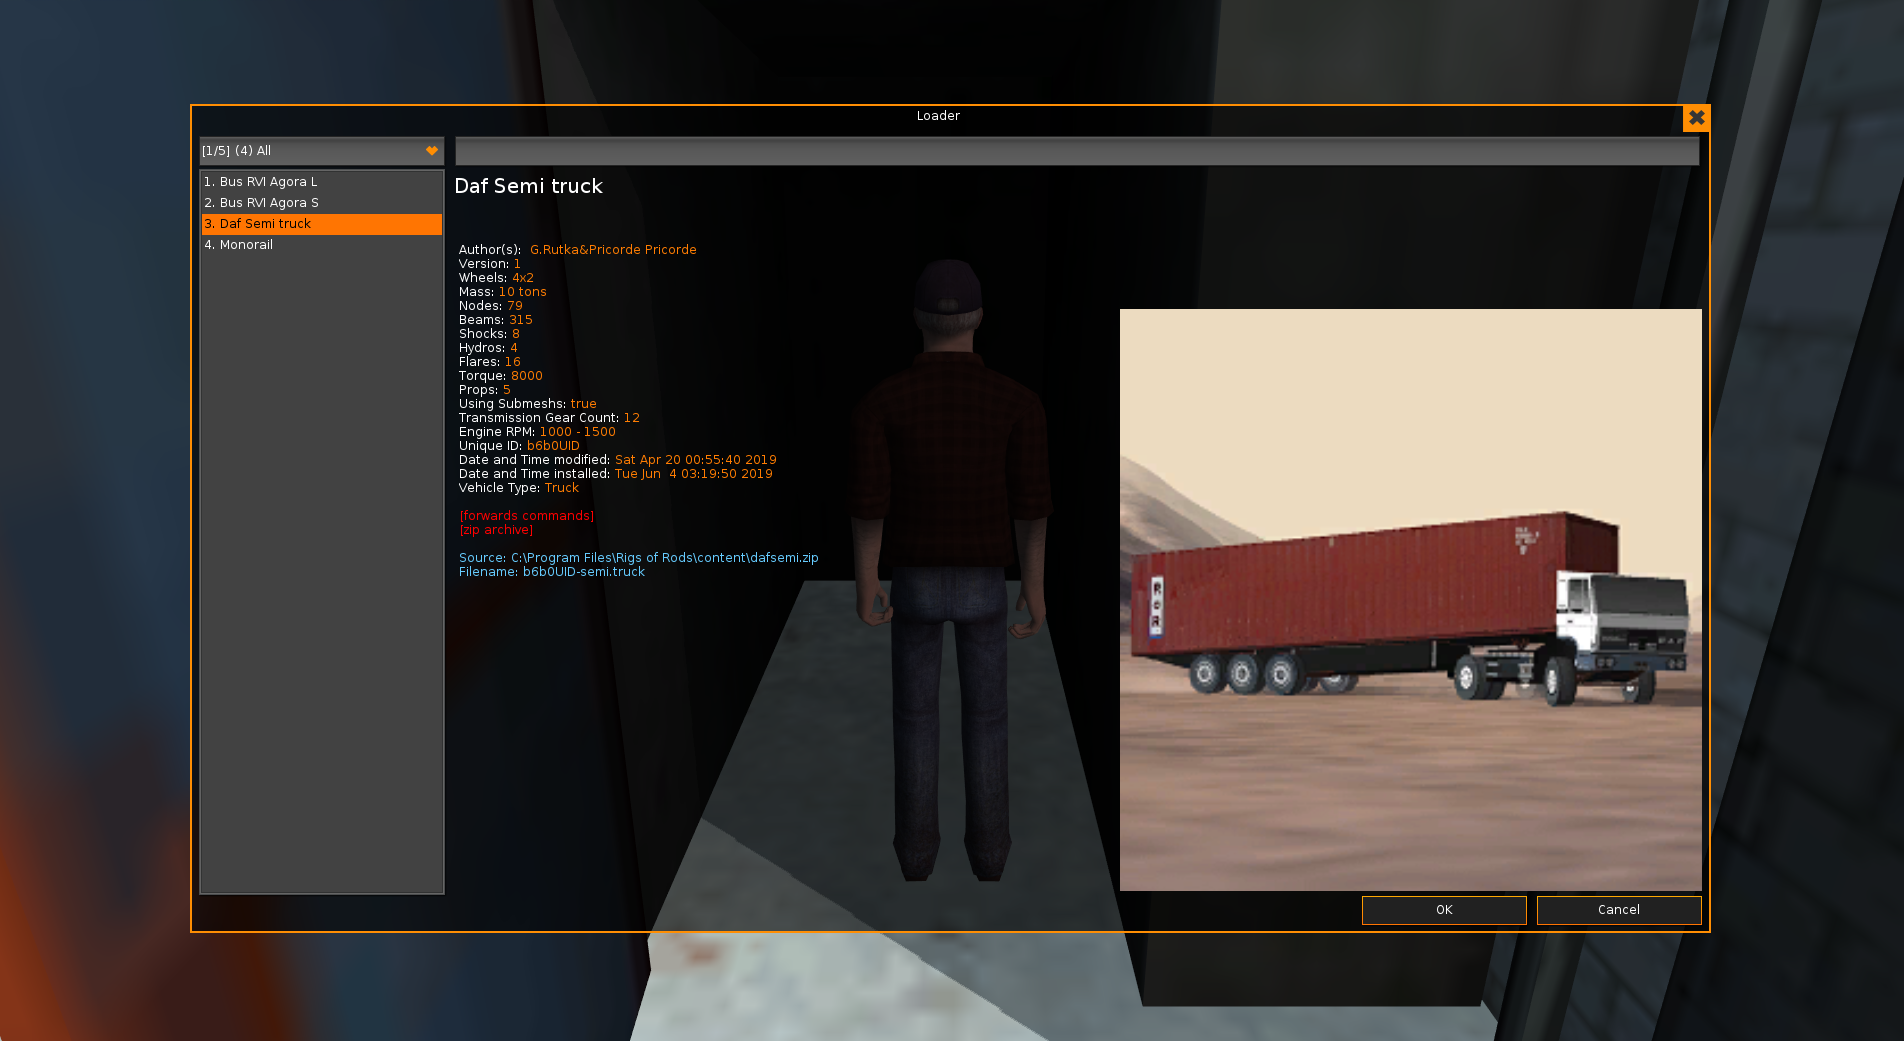
\includegraphics{images/bg-vehselect.png}

Use the mouse or arrow keys to move through the menus. Select the
\emph{DAF Semi truck}. The truck spawns inside the Rig-a-Deal with you
inside it. If you happen to spawn the truck with RoRBot outside of the
vehicle, simply hit \texttt{ENTER}/\texttt{RETURN} to get in a vehicle.

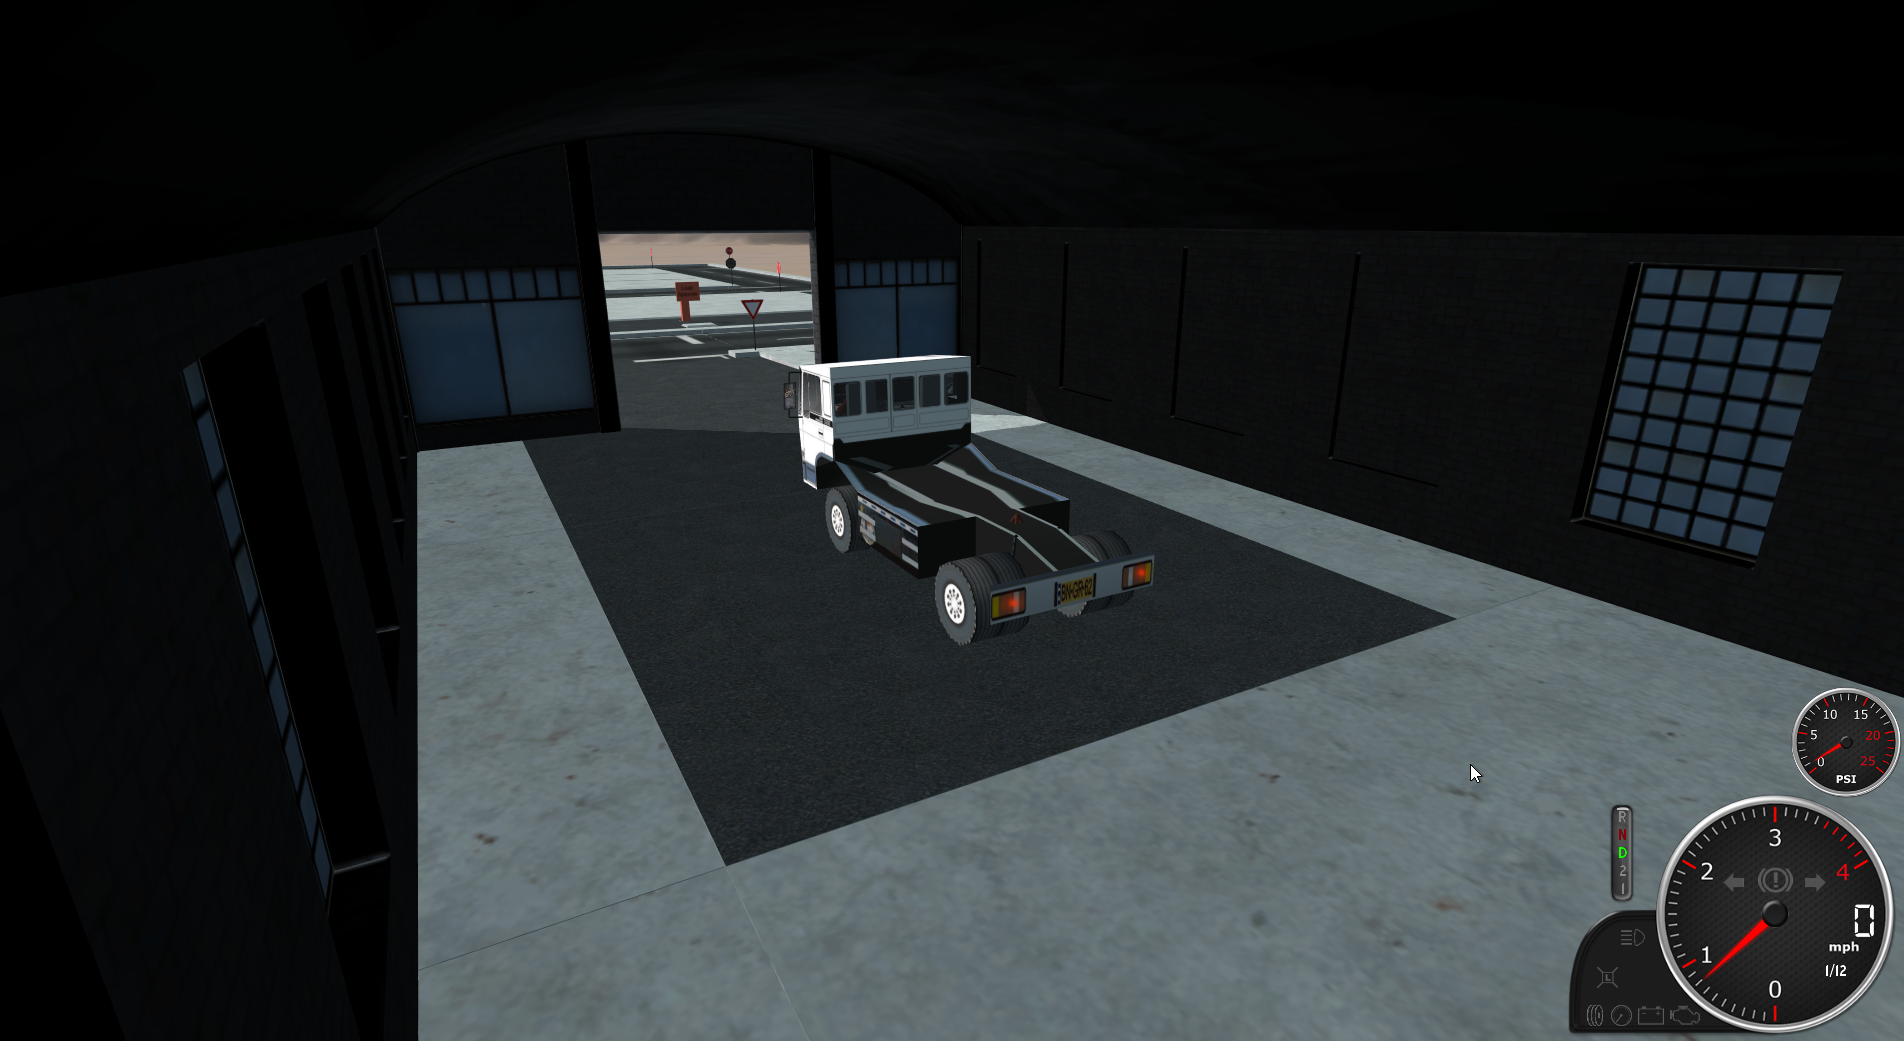
\includegraphics{images/bg-daf1.png}

\hypertarget{driving}{%
\section{Driving}\label{driving}}

The DAF semi isn't the most agile or best looking truck in the game, but
it serves us a purpose later. The camera inside the Rig-a-Deal is fixed,
so you will be unable to move it until you leave. Switch to the in-cab
camera by hitting \texttt{C}. Use the \texttt{UP} arrow key to
accelerate out of the \emph{Rig-a-Deal} (Rigs of Rods uses a simulated
clutch which begins to engages at a specific point. This why the semi
doesn't move until 1000 RPM). Use \texttt{DOWN} to brake, and
\texttt{LEFT}/\texttt{RIGHT} arrows to steer. Use
\texttt{PGUP}/\texttt{PGDOWN} to select your transmission
direction/speed.

Start by exploring Coldwater, the town you begin in. It isn't very big
but provides some decent moving room. If you get stuck, or wreck, hit
\texttt{I} to reset back to the \emph{Rig-a-Deal}, or \texttt{BACKSPACE}
to reset the truck in its current position.

If you hold \texttt{BACKSPACE} for one second, you will enable the
``advanced repair mode'' which lets you move the vehicle to any position
by using the \texttt{WASD} keys to move and the arrow keys to rotate.
Press \texttt{BACKSPACE} again to exit.

You can switch transmission modes by hitting \texttt{Q}. There are 5
transmission modes available: * Automatic shift * The gear change is
fully automatic, the player only has to set the gear by pressing
\texttt{PGUP}/\texttt{PGDOWN}. * Manual shift: Auto clutch * The gear is
changed on user request. No clutch should be pressed to change gear,
vehicle takes care of that. Just use \texttt{A} and \texttt{Z} to shift.
* Fully manual: sequential shift * The user must press clutch and select
whether it is needed to switch up or down. Depress the clutch by hitting
\texttt{LEFT\ SHIFT}, then press \texttt{A} to upshift or \texttt{Z} to
downshift. * Fully manual: stick shift * This mode is useful if you have
a game controller with an H-shifter (like Logitech G27). In this mode
the player can set gears 1-6, N, and R directly by the stick. * Fully
manual: stick shift with ranges * This mode is mostly used in vehicles
having more gears than 6. In this case you can select from 3 ranges: low
(gear 1-6), medium (gear 7-12), high (gear 13-18) by pressing the
appropriate button. Like if you want to select the 8th gear, you have to
select gear N first, press the midrange button, then select the 2nd gear
on the h-stick. Remember, range selection can be made only if the gear
is in N.

If you stall, there are 2 keys to be remembered: \texttt{X} enables or
disables the electricity in the vehicle, and \texttt{S} activates the
starter. Press \texttt{X} and you'll see a yellow battery icon lit on
the UI. Hold \texttt{S} until the engine is started. Resetting the
vehicle with \texttt{BACKSPACE} or \texttt{I} will instantly start the
engine.

Remember how to change the camera? Hit \texttt{C} twice. You're now in
third-person view and can move the camera around. Use the number pad
(specifically \texttt{2}, \texttt{4}, \texttt{6}, and \texttt{8}) to
move the camera. Pressing \texttt{5} resets the camera. \texttt{9} and
\texttt{3} zoom in/out respectively and \texttt{1} gives you a front
view of your truck.

You can also move the camera by holding right-click and dragging with
your mouse.

Now, make your way back to the \emph{Rig-a-Deal}.

\hypertarget{trailer-loads}{%
\section{Trailer Loads}\label{trailer-loads}}
You should see a large, grey, open-platform with an orange console. Park
the truck (use \texttt{P} to set the parking brake) and hit
\texttt{ENTER}/\texttt{RETURN} to get out. Note that the same camera
commands work with RoRBot. Step in front of the orange console to open
the load selector.

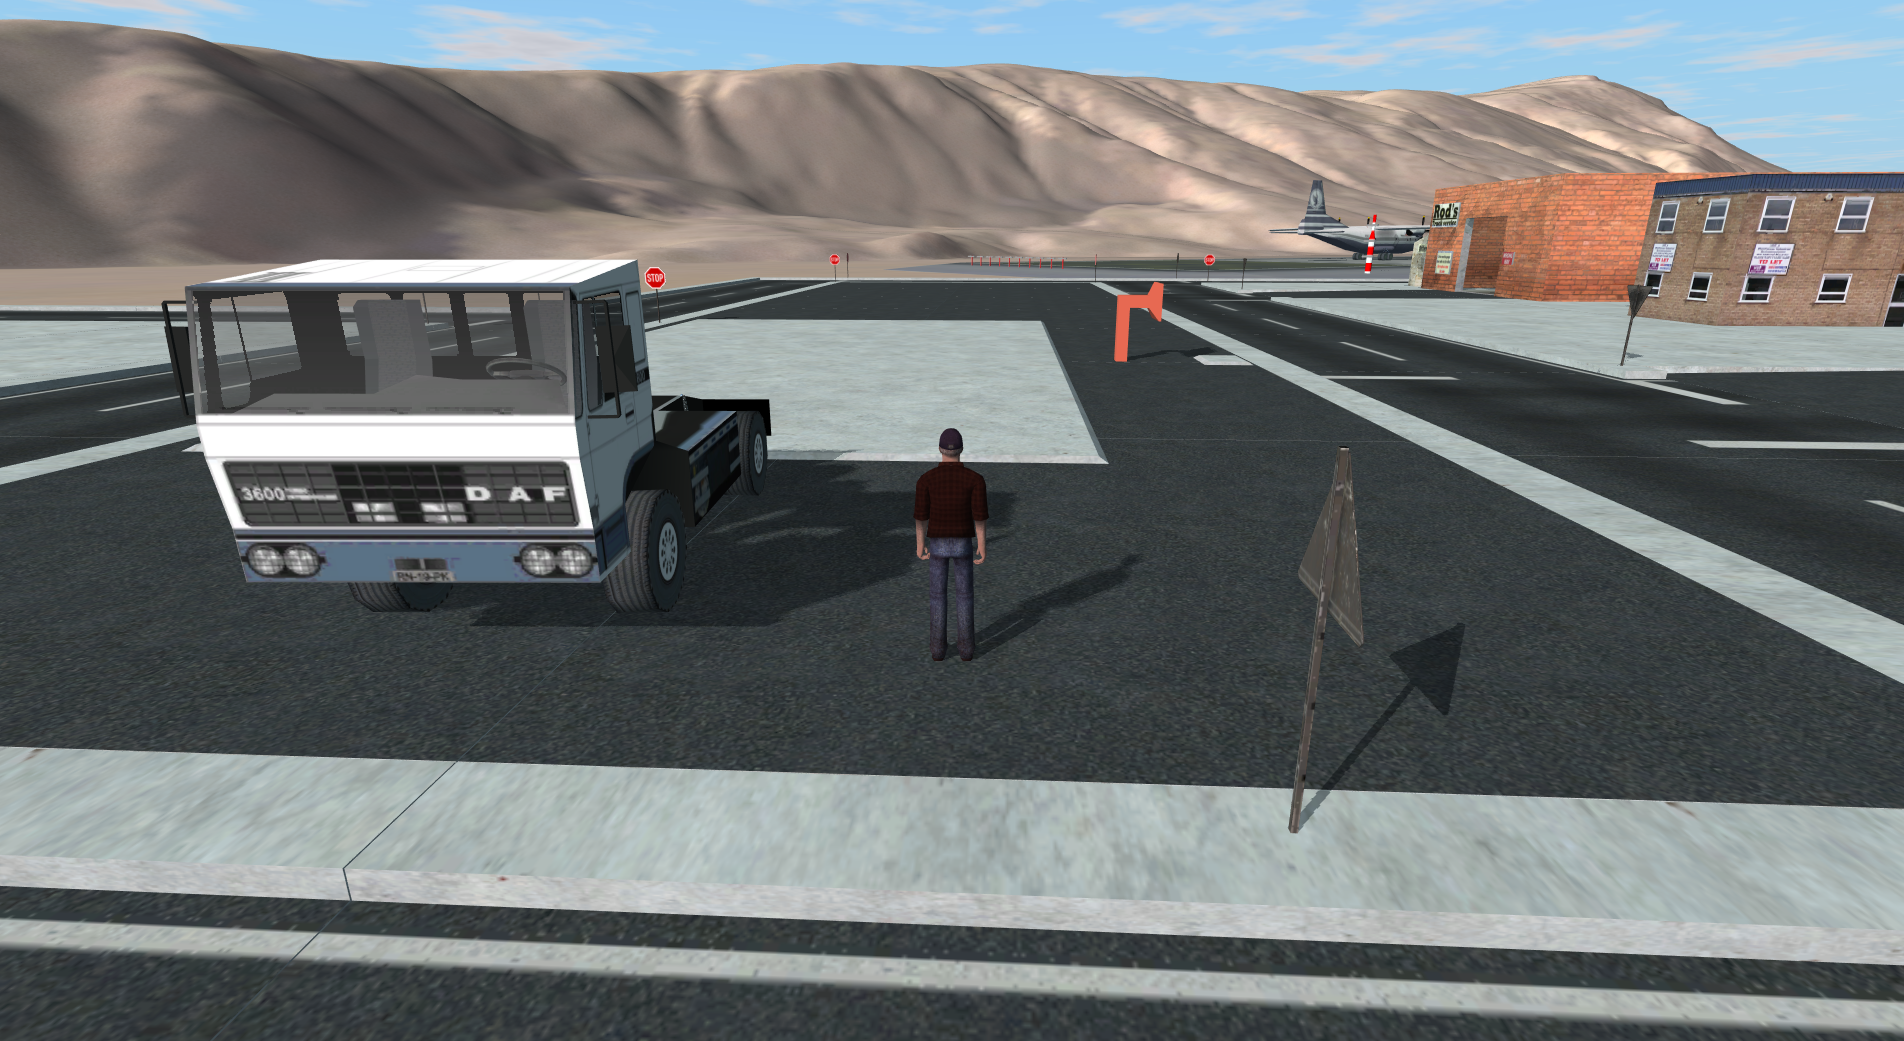
\includegraphics{images/bg-daf2.png}

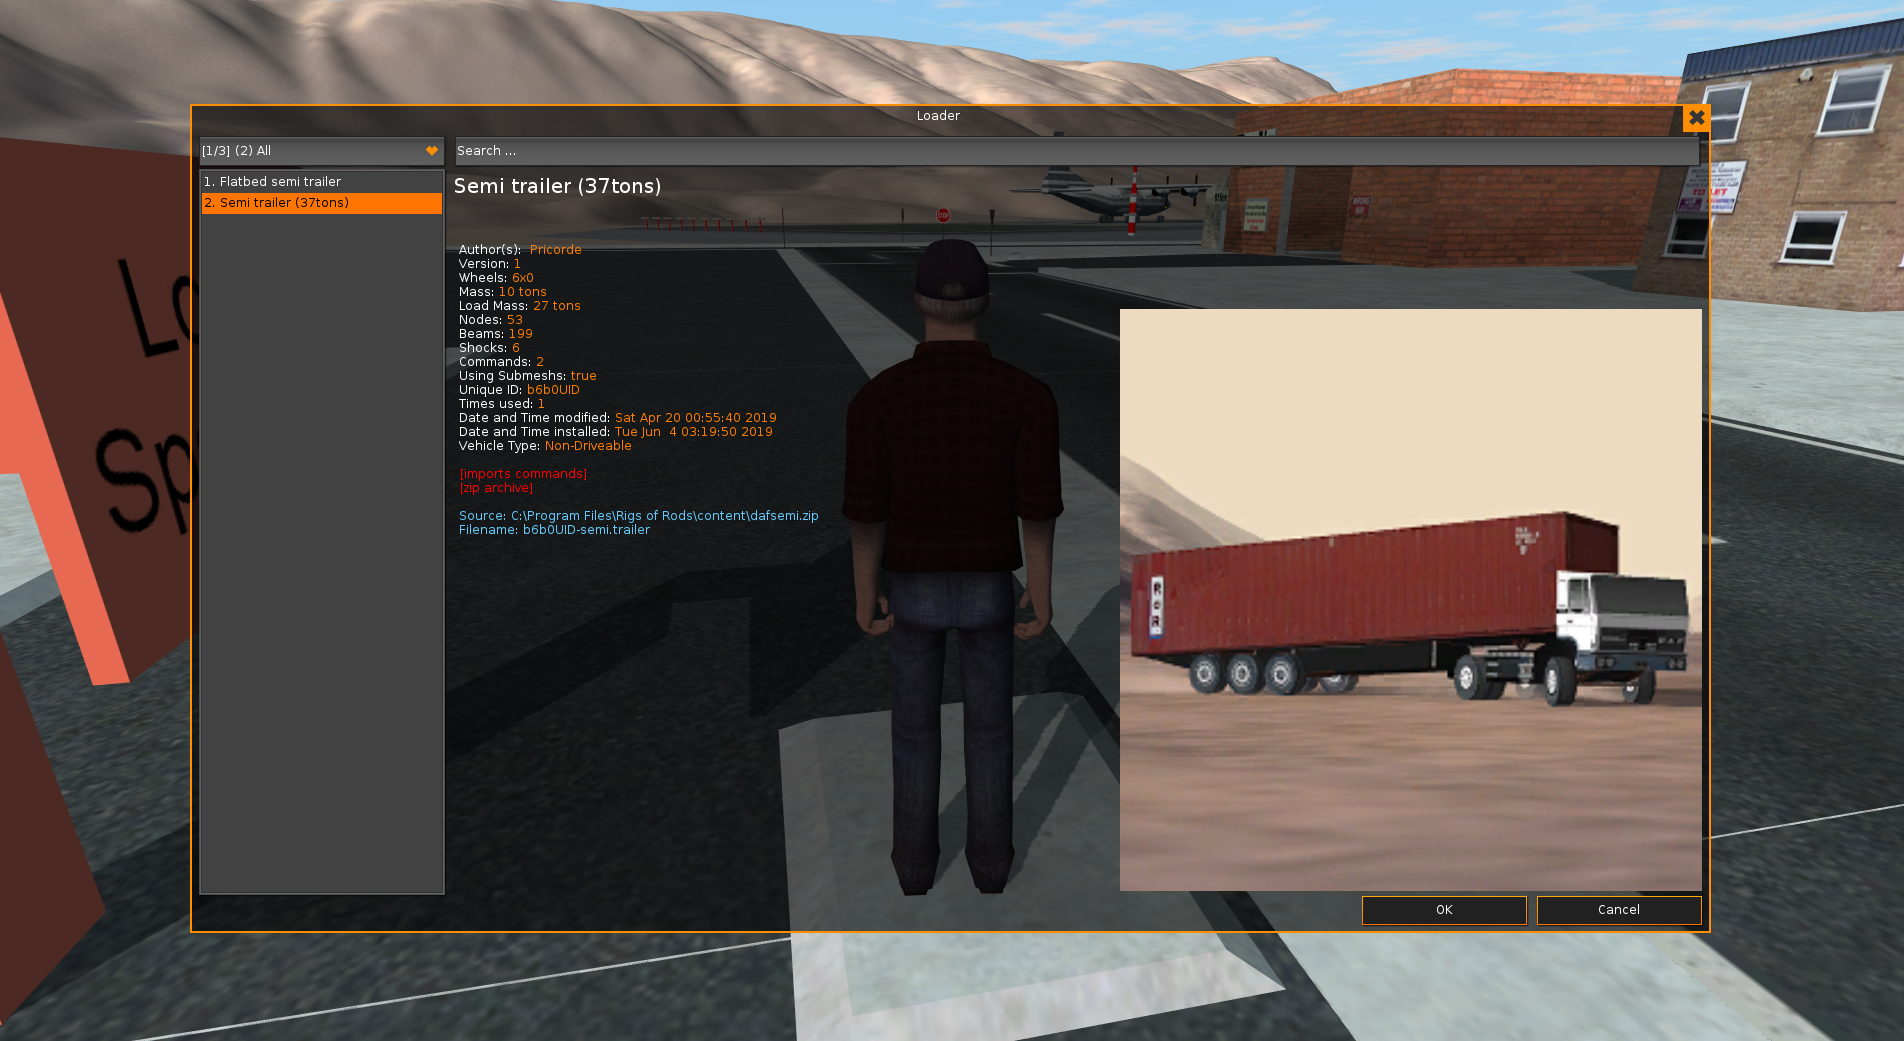
\includegraphics{images/bg-loadselect.png}

Select the \emph{Semi trailer (37 tons)}.

Get back in the semi and drive in front of the load. Use the camera in
third-person view to help you if you need. Back into the trailer. When
you get close, use \texttt{F1}/\texttt{F2} to lower and raise the
trailer legs respectively.

The hook points must be within 10cm to hook, so it may take some
practice to get close. When you think you're close, hit \texttt{L}. If
you're close enough, the semi will latch to the trailer. Raise the legs
by holding \texttt{F1}.


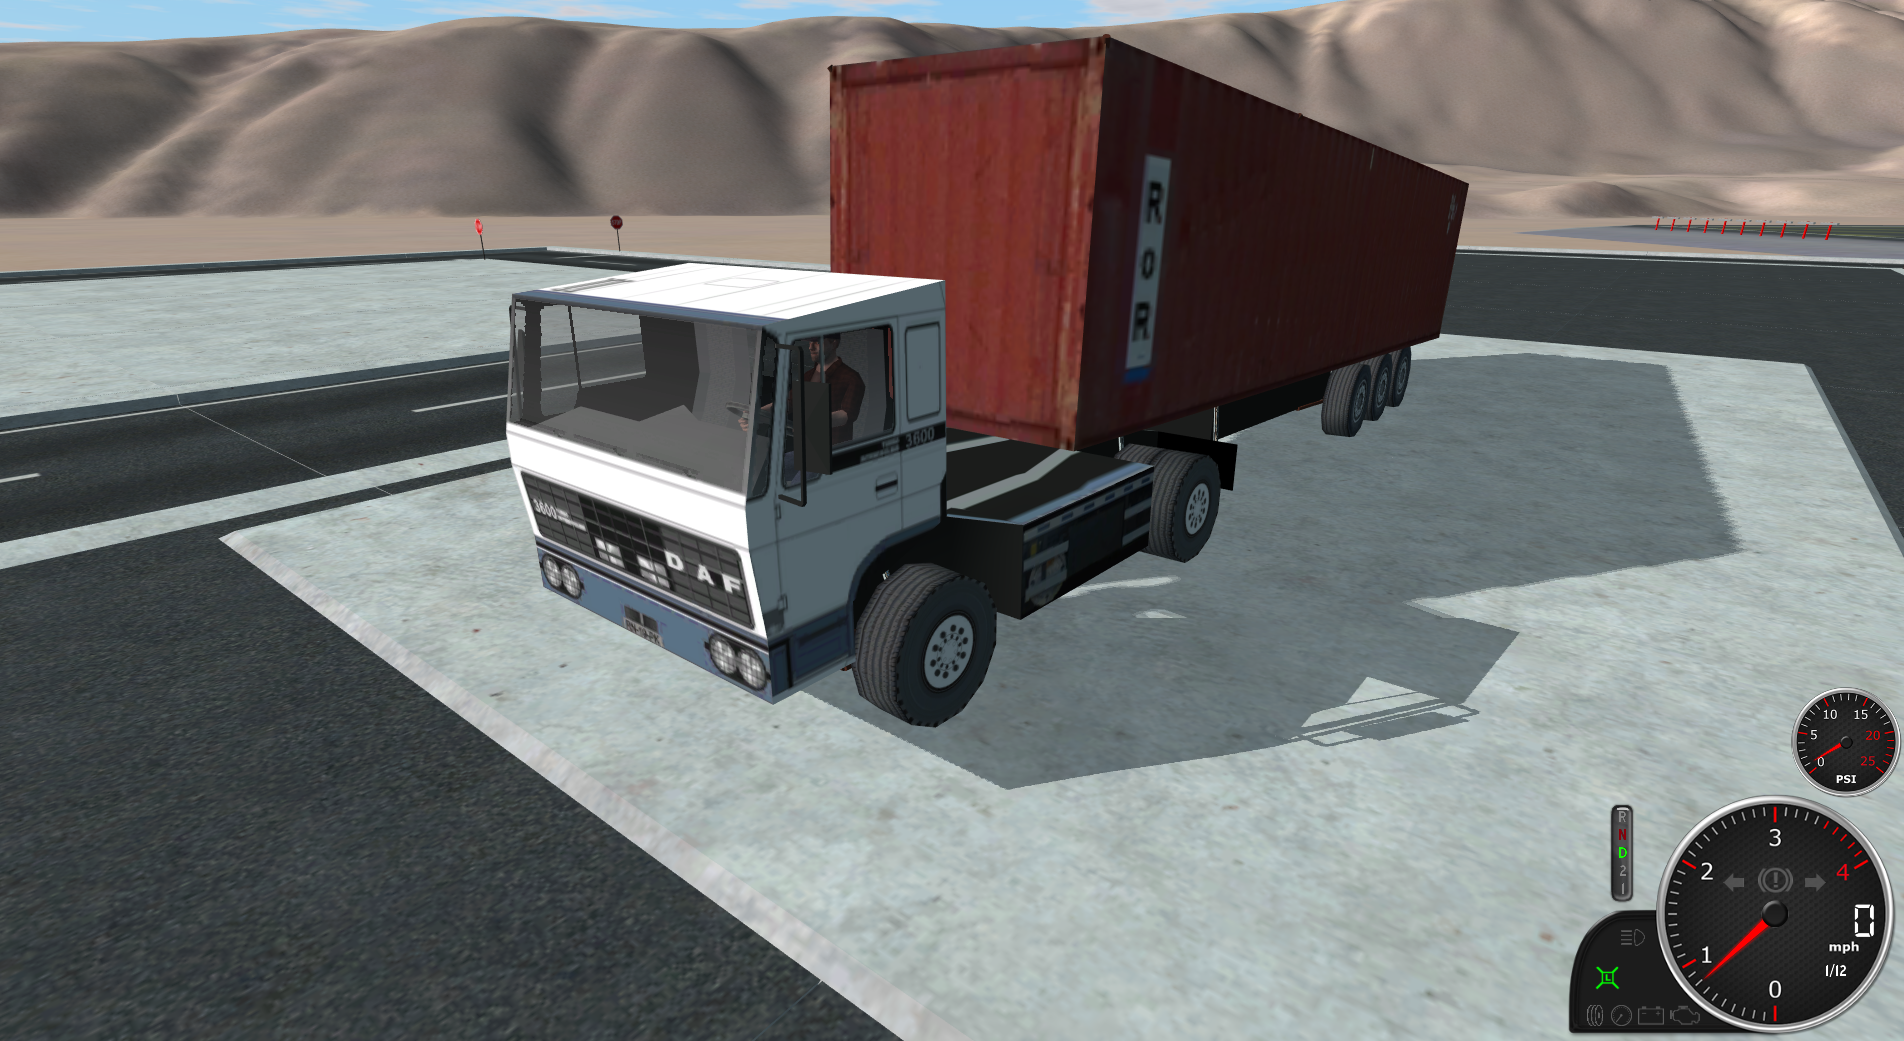
\includegraphics{images/bg-daf3.png}

You can now drive around with the trailer. You will notice that the
trailer has a large effect on how the semi pulls and handles! This
process is the same for most trailers. In some cases you can secure
loads to trucks using \texttt{O}.

NOTE: on some computers trailers may increase lag or decrease FPS(frames
per second) dramatically!

\hypertarget{flying}{%
\section{Flying}\label{flying}}

Now that we've become comfortable with driving. Let's try to fly. Move
your mouse to the to top of the screen to bring up the menubar, click
\texttt{Vehicles} then \texttt{Antonov\ 12} to instantly enter the plane
which is sitting on the runway.


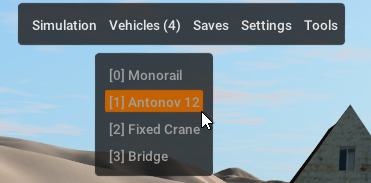
\includegraphics{images/bg-planeselect.png}


Apply the parking brake by pressing \texttt{P}. Turn on the flying
lights by pressing \texttt{M}. Start the engines by using your mouse to
click the \texttt{ON} buttons in the lower right hand corner (or by
pressing \texttt{CTRL+HOME}).

When the engines settle to the appropriate idle speed (somewhere near
750rpm), release the parking brake and throttle the engines to full by
holding \texttt{PGUP}. Pressing \texttt{CTRL+PGUP} will instantly set
the throttle to max.

If you have a short runway, be sure to use the flaps with \texttt{1} and
\texttt{2} (this is especially helpful in multiplayer). When you reach
75-80 knots, lift up by pressing the \texttt{DOWN} arrow. Steer with the
\texttt{LEFT}/\texttt{RIGHT} arrows and control the rudder with
\texttt{Z} and \texttt{X}. Raise the landing gear, in this plane, by
holding \texttt{F3}.

The An-12 does not stand high speeds (175+ knots) well, and you may find
that if you go too fast the wings will break apart!

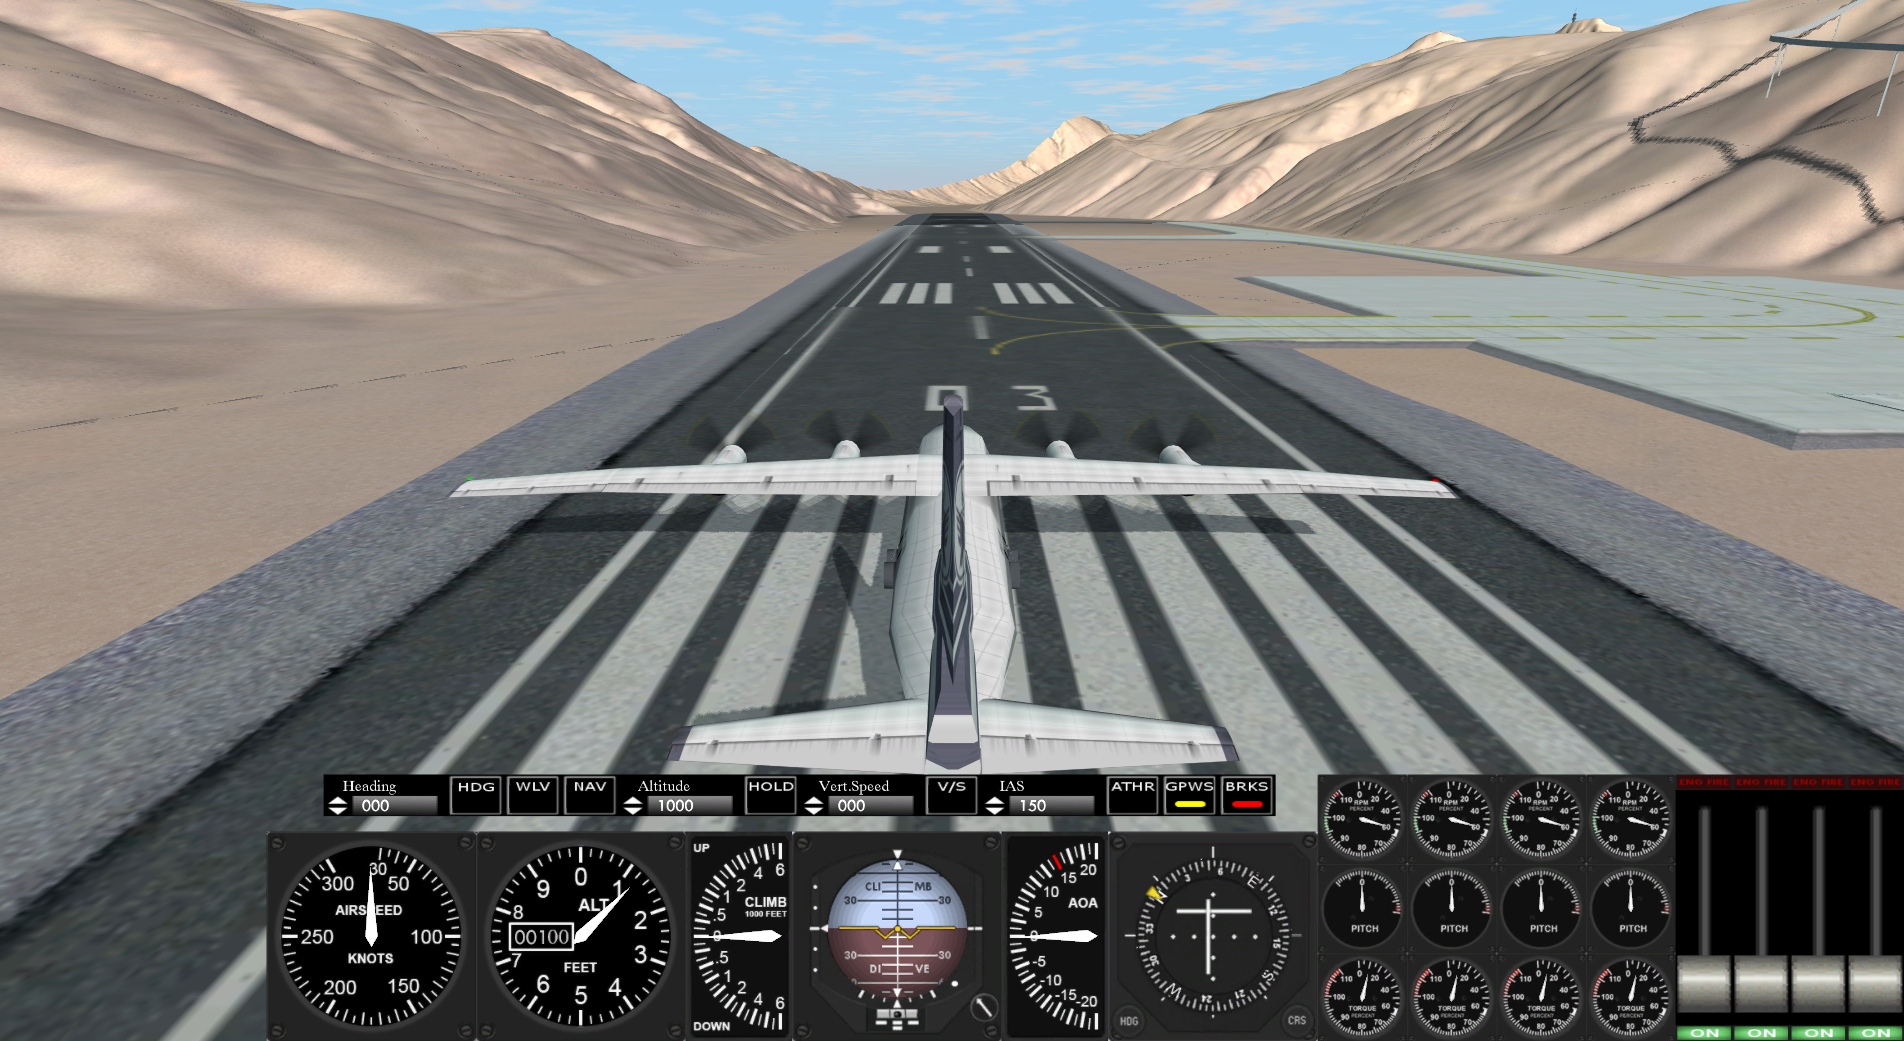
\includegraphics{images/bg-plane1.png}

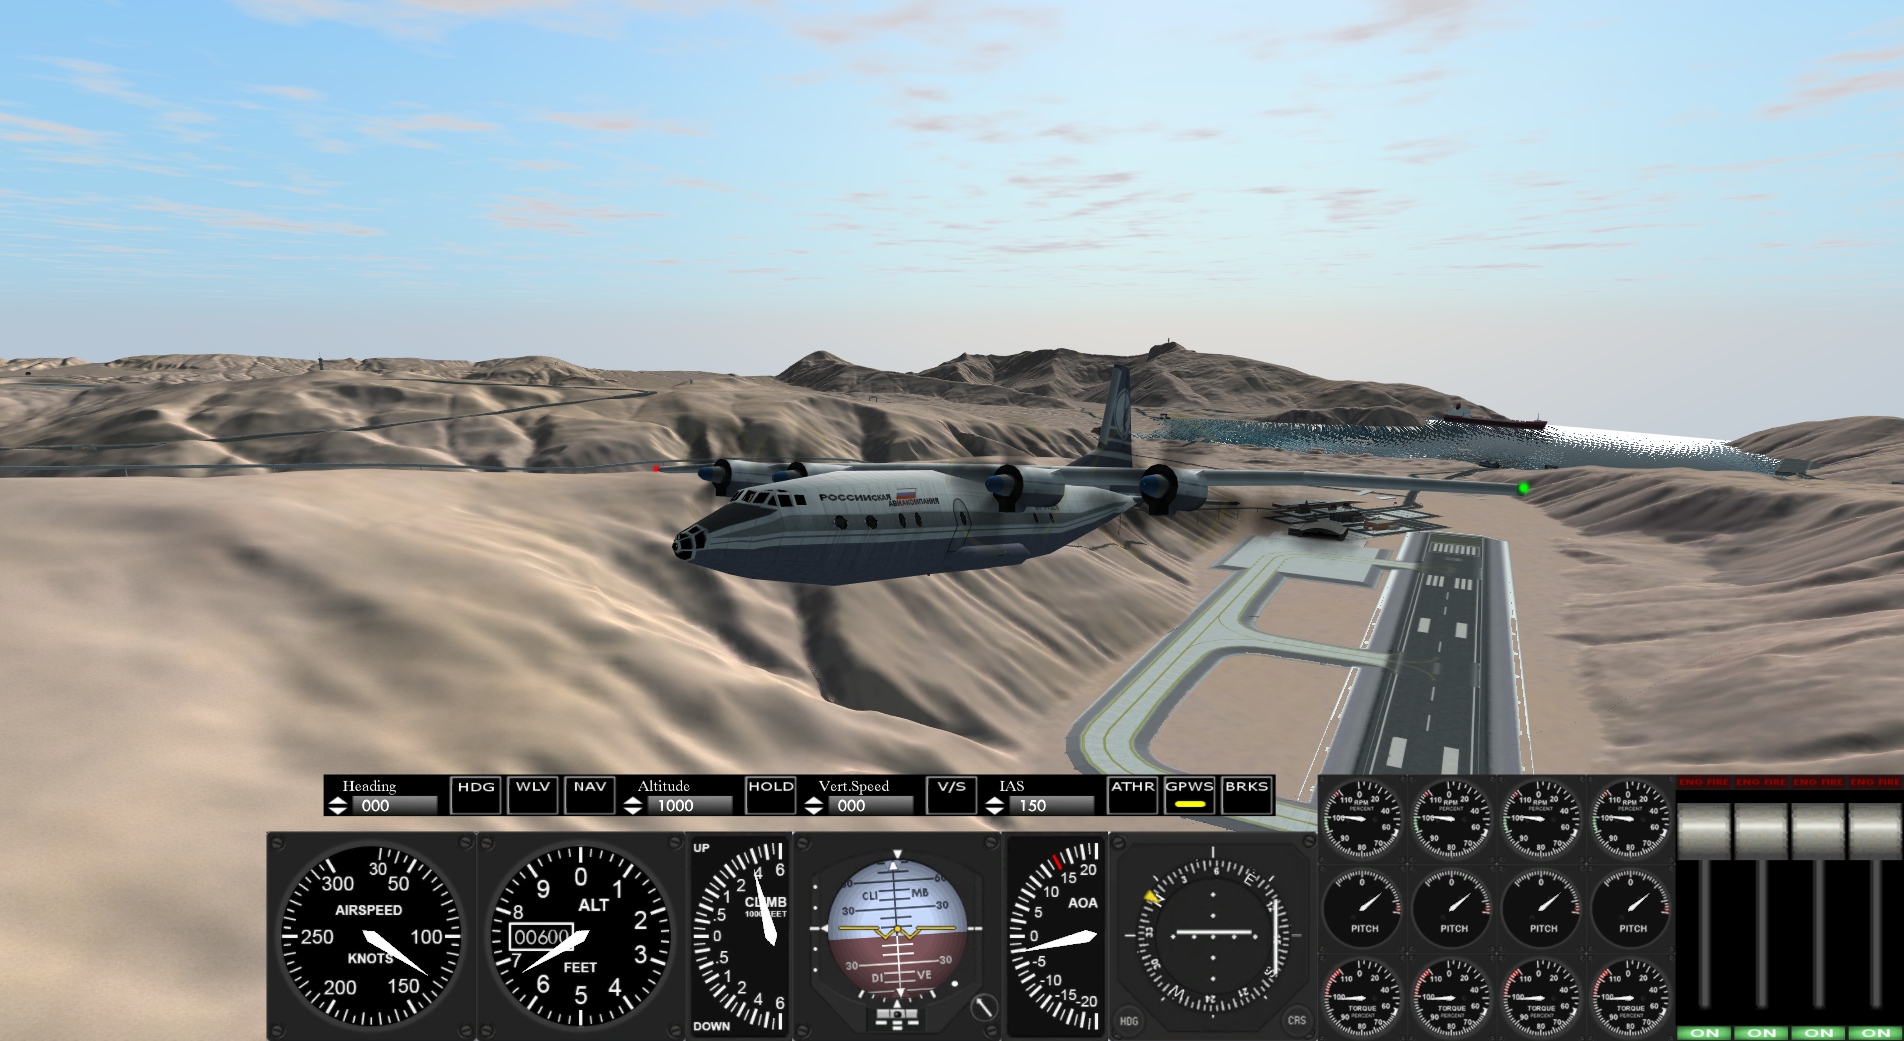
\includegraphics{images/bg-plane2.png}

When it comes to landing, make sure you have room to slow down and take
your time. Going straight into the runway is the easiest way to land
when you first start off. It may take a few passes to go head-on so
don't be afraid to abort a landing and throttle back up to regain
altitude. The entire process is easier if you shadows enabled, but is
possible without. When you land, hit \texttt{R} to reverse thrust and
throttle up to slow down in addition to using \texttt{B} to brake the
wheels.

This tutorial does not make use of the autopilot. For more information
regarding the use of autopilot, see
\href{/gameplay/aircraft-handling/}{Aircraft handling}.

\hypertarget{boating}{%
\section{Boating}\label{boating}}

We must explore beyond Coldwater to get to the marina. Take the main
road out of Coldwater, heading southwest toward the Elk Hotel. Take the
second left after you leave town. You should see the water soon. When
you arrive at the marina, you should see marina-style boat docks and a
ramp along with a building.

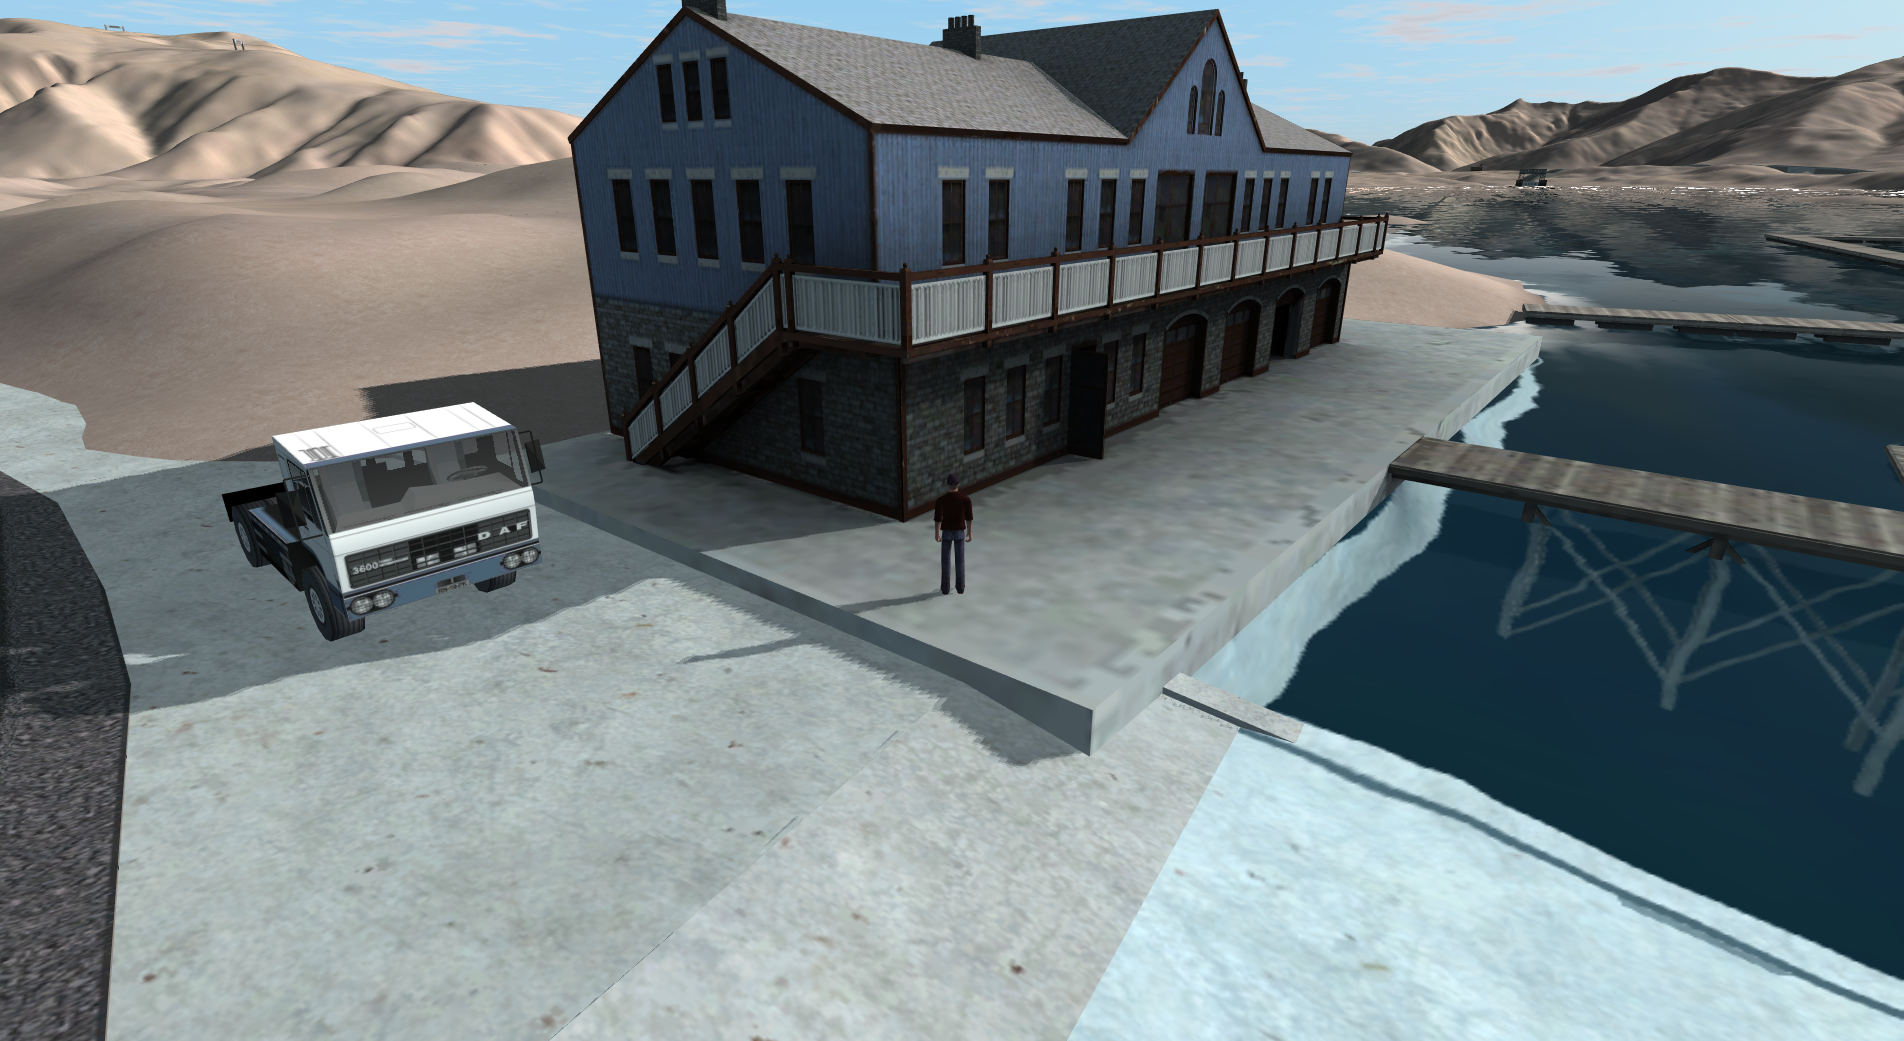
\includegraphics{images/bg-boat1.png}

Walk around to the front of the building and enter the open door. Choose
the Wahoo boat.

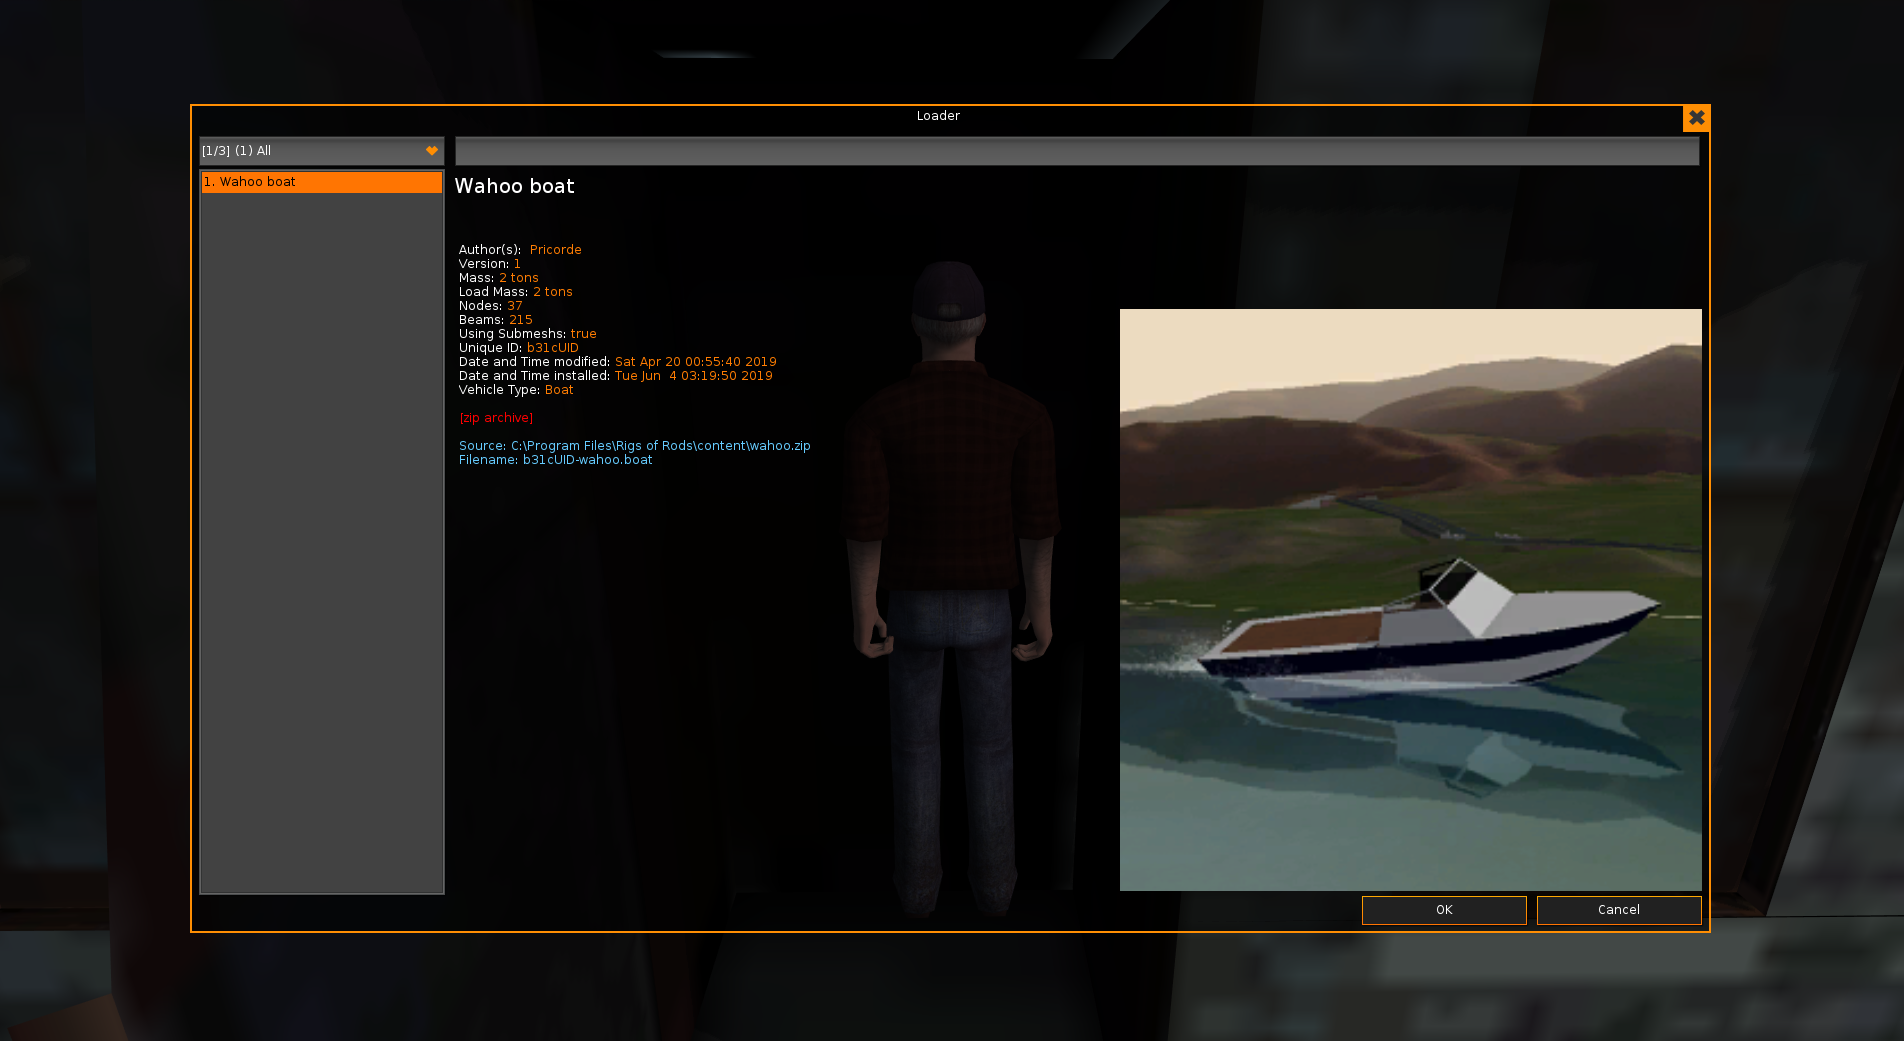
\includegraphics{images/bg-boatselect.png}

Use \texttt{UP}/\texttt{DOWN} to throttle and
\texttt{LEFT}/\texttt{RIGHT} to steer. Use \texttt{PGUP} to center the
throttle (to neutral) and \texttt{PGDOWN} to center the rudder. It may
take you a while to get your sea legs. If you have waves enabled, see
how far out you can go before you flip over waves!

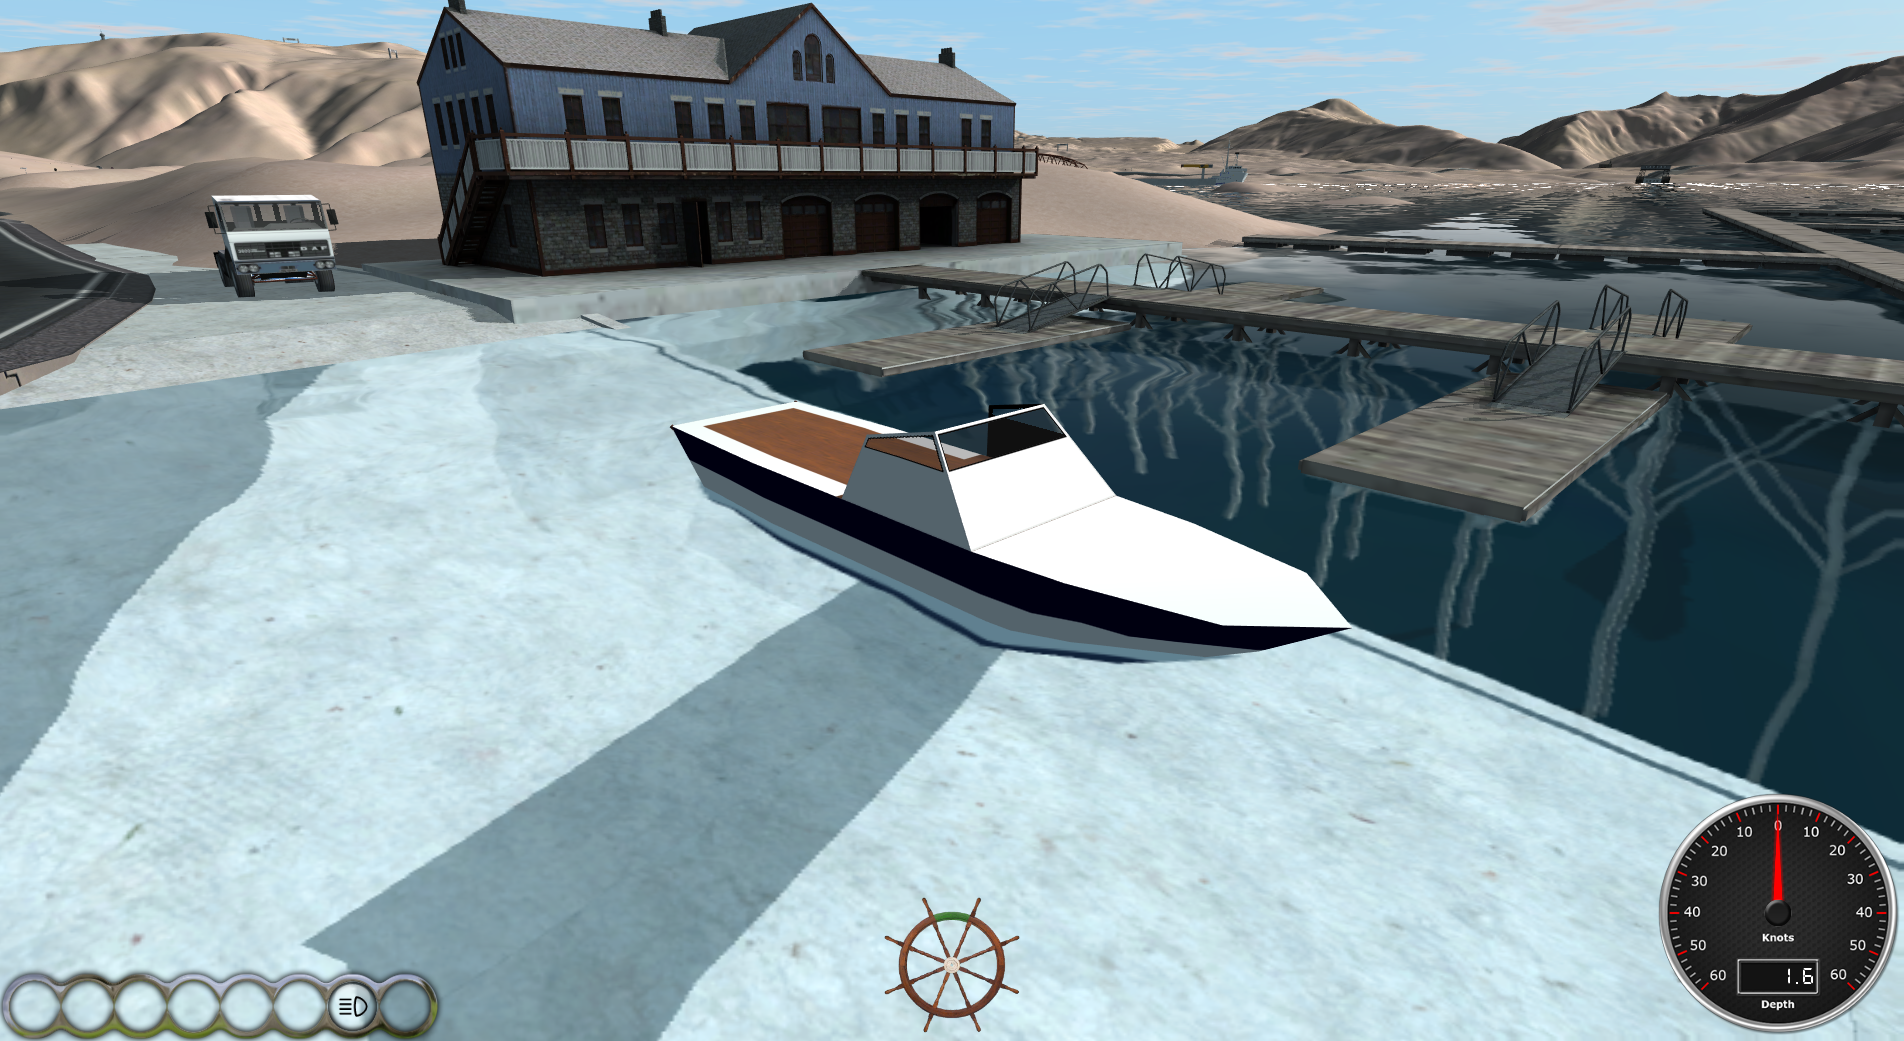
\includegraphics{images/bg-boat2.png}

\hypertarget{conclusion}{%
\section{Conclusion}\label{conclusion}}

Now that you have a basic grasp of the basic vehicles in RoR, it is now
up to you to create your own scenarios. If you feel bored, try the vast
selection of mods available on the
\href{https://forum.rigsofrods.org/resources/}{Repository}.

\hypertarget{multiplayer}{%
\section{Multiplayer}\label{multiplayer}}

If you feel like sharing the experience, you can play on one of the many
public multiplayer servers. To get started, click the
\texttt{Multi\ player} button on the main menu.

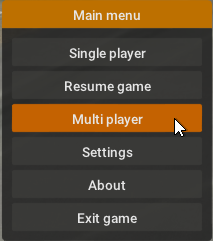
\includegraphics{images/bg-mp1.png}

Set your username by clicking on \texttt{Settings} and changing it in
the \texttt{Player\ nickname} textbox.

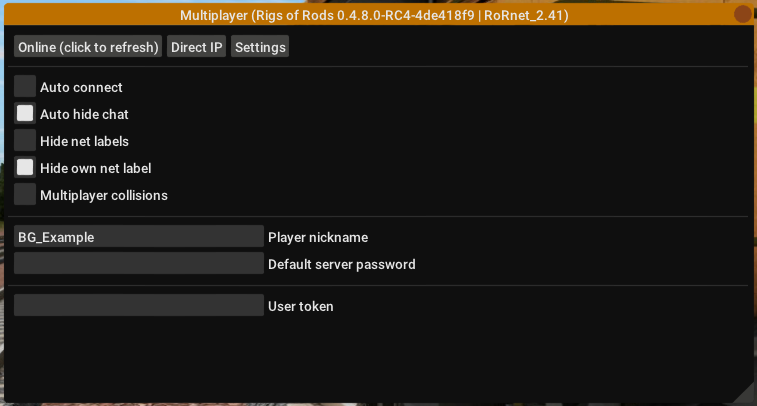
\includegraphics{images/bg-mp2.png}

You may have to restart the game for the changes to take effect.

Now just select the server you want to play on, then click
\texttt{Join}.

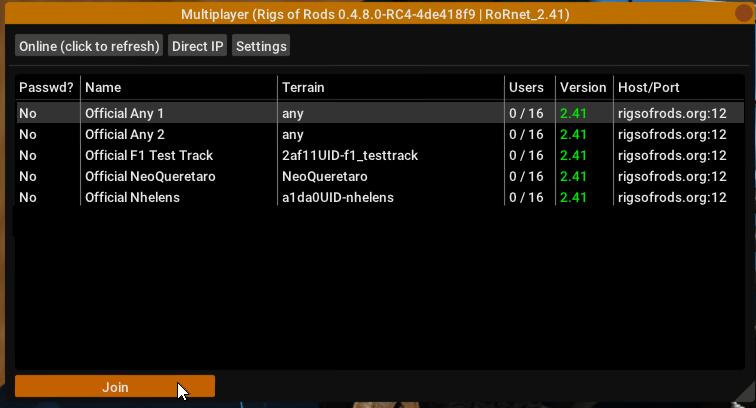
\includegraphics{images/bg-mp3.png}
The `any' servers allow you to select a terrain, while other servers
(such as Official Nhelens) are set to use a specific terrain.
While on a server, you can enable collisions between other players or
hide nicknames by going to \texttt{Settings} in the top menubar.

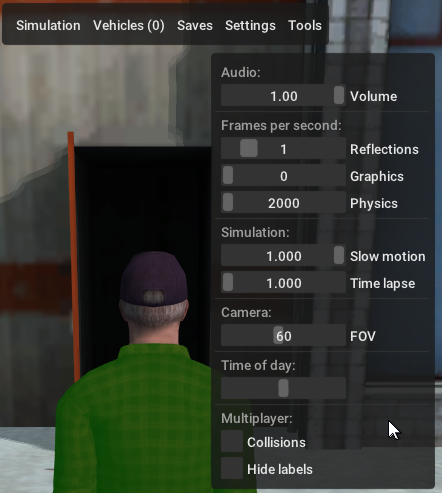
\includegraphics{images/bg-mp4.png}

Note that multiplayer is still in development and can be unstable at
times!
